\documentclass[11pt]{article}
\usepackage[english]{babel}
\usepackage[utf8]{inputenc}
\usepackage{fancyhdr}
\usepackage{graphicx}

\def\Name{Ran Liao}
\def\Topic{Activity Diagram}

\title{\textbf{\Topic}}
\author{\Name}
\markboth{Notes on \Topic\ }{Notes on \Topic\ }
\date{\today}
 
\pagestyle{fancy}
\fancyhf{}
\rhead{\date{\today} }
\lhead{Notes on \Topic\ }
\rfoot{\thepage}

\textheight=9in
%\textwidth=6.5in
\topmargin=-.75in
%\oddsidemargin=0in
%\evensidemargin=0in
 
\begin{document}
\maketitle
\noindent\makebox[\linewidth]{\rule[8pt]{5in}{0.5pt}}

\section*{Overview}

An activity diagram shows how events that occur at the same time are coordinated. It is used when activities are carried on in parallel.

\section*{Terminology}

\begin{itemize}

	\item \textbf{Fork}
	
	A fork has one incoming transition, and many outgoing transitions, each of which starts an activity to be executed in parallel with the other activities.
	
	\item \textbf{Join}
	
	A join has many incoming transitions, each of which lead from an activity executed in parallel with the other activities, and one outgoing transition that is started when all the parallel activities have been completed.
	
\end{itemize}

\begin{figure}[h]
	\centering
	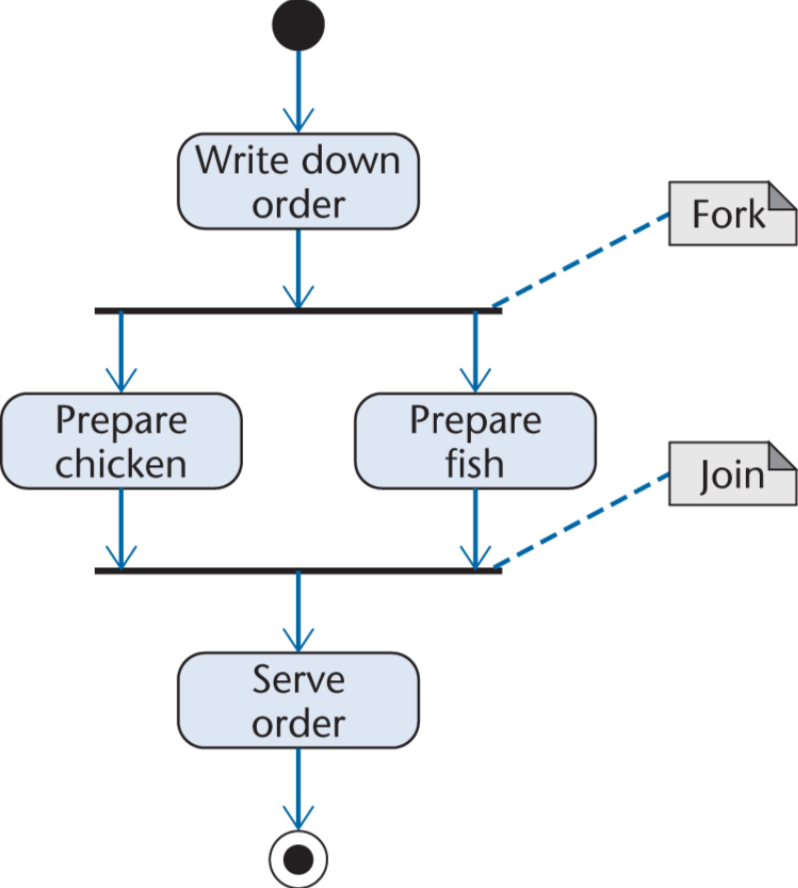
\includegraphics[width=0.45\linewidth]{images/ActivityDiagram.png}
	\caption{Activity Diagram}
	\label{fig:ActivityDiagram}
\end{figure}


\end{document}